%# -*- coding: utf-8 -*-
\documentclass{beamer}
\usepackage[bars]{beamerthemetree}
\usetheme{Darmstadt}
%\usecolortheme{lily}
%\usecolortheme{sidebartab}
\usestructuretemplate{\color{structrue}}{}
\beamertemplateshadingbackground{magenta!5}{blue!5}

\usepackage{xeCJK}
\usepackage{mathrsfs}
\usepackage{latexsym}
\setCJKmainfont[BoldFont=SimHei]{SimSun}
\usefonttheme[onlymath]{serif}
\usepackage{moreverb}

\usefonttheme{structurebold}
\usepackage{amsmath,amssymb}

\title{分离逻辑定理证明器的设计与实现 \\ 中期检查报告}
\author{PB09210183 何春晖}
\date{2013年 5月 7日}

\begin{document}
\frame{\titlepage}

%\frame{\frametitle{目录}\tableofcontents}
%\AtBeginSection[]
%                  {
%                    \begin{frame}<beamer>
%                      \frametitle{目录}
%                      \tableofcontents[currentsection]
%                    \end{frame}
%                  }
\section{选题背景}
\begin{frame}[fragile]
  \begin{block}{背景}
    \begin{itemize}
    \item 分离逻辑是一种处理可变数据结构的逻辑
    \item 为提高验证可信度,要产生机器可检查的证明
    \item 需要一定的自动化
    \end{itemize}
  \end{block}
  \pause
  \begin{block}{现有证明器不能完全满足需要}
    \begin{columns}
      \begin{column}{0.45\textwidth}
        交互式证明器(Coq等):
        \begin{itemize}
        \item 易支持分离逻辑
        \item 证明能够被事后检查
        \item 自动化较差
        \end{itemize}
      \end{column}
      \begin{column}{0.45\textwidth}
        SMT证明器(Z3等):
        \begin{itemize}
        \item 不支持分离逻辑
        \item 证明难以被事后检查
        \item 完全自动化
        \end{itemize}
      \end{column}
    \end{columns}
  \end{block}
  \pause
  \begin{block}{结论}
    实现一个{\color{red}能够输出Coq证明}的SMT证明器,同时{\color{red}加入分离逻辑的验证}功能。
  \end{block}
\end{frame}

\section{已完成的工作}
\begin{frame}[fragile]
  \begin{block}{总体结构}
    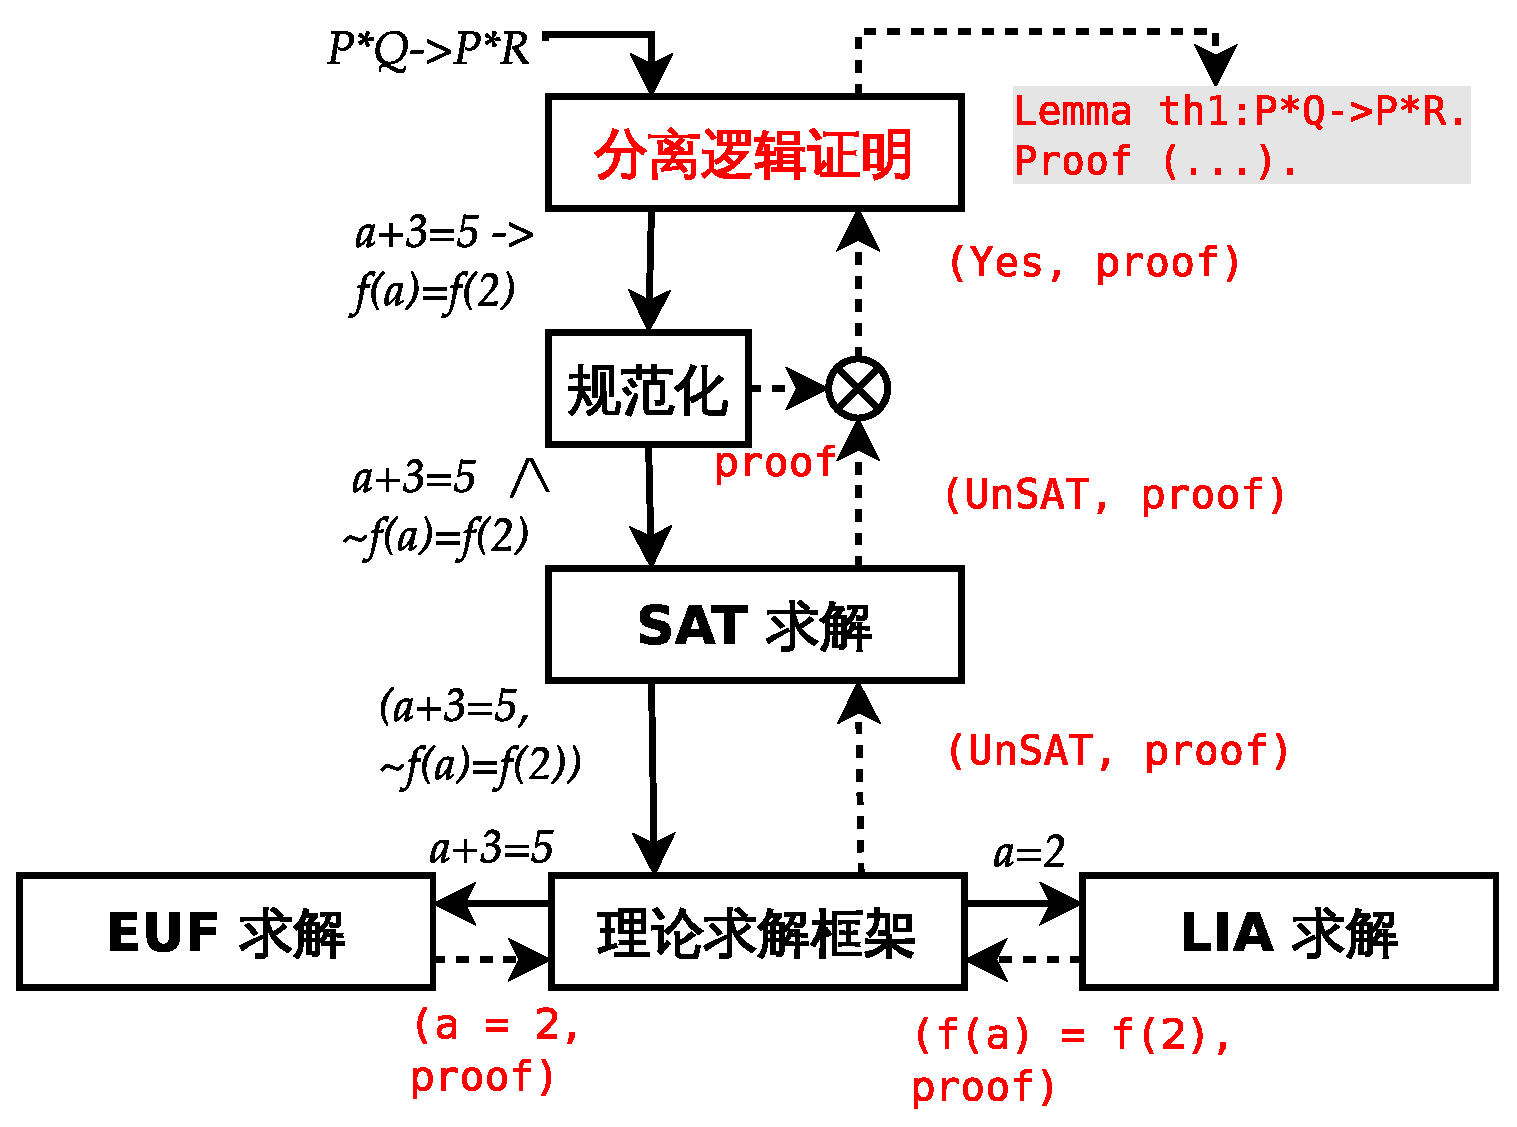
\includegraphics[width=0.8\textwidth]{stru.eps}
  \end{block}
  \begin{block}{}
    基本完成输出Coq证明的工作
  \end{block}
\end{frame}

\begin{frame}[fragile]
  \begin{block}{规范化}
    将待证命题的否定转换为CNF范式
  \end{block}
  \begin{block}{}
    \begin{tabular}{c|rcl}
      步骤 & 引用的定理 & & \\
      \hline
      否定 & & &\\
      \hline
      消蕴含 & $P \rightarrow Q$ & $\leftrightarrow$ & $\lnot P \lor Q$  \\
      \hline
       & $P \lor Q$ & $\leftrightarrow$ & $\lnot ( \lnot P \land \lnot Q )$ \\
      消否定 & $ P \land Q$ & $\leftrightarrow$ & $\lnot ( \lnot P \lor \lnot Q )$ \\
      & $ \lnot \lnot P$ & $\leftrightarrow$ & $P$ \\
      \hline
      $\lor$对$\land$分配 & $ P \lor (Q \land R)$ & $\leftrightarrow$ & $(P \lor Q) \land (P \lor R)$ \\
    \end{tabular}
  \end{block}
  \begin{block}{}
    例:
    $$ P \land ( P \rightarrow Q ) \rightarrow Q \longmapsto P \land (\lnot P \lor Q) \land \lnot Q $$
  \end{block}
\end{frame}

\begin{frame}[fragile]
  \begin{block}{SAT求解}
    寻找可能使命题成假的模型 \\
    得到$\lnot \alpha \rightarrow \mathrm{False}$的证明。\\
    依反证律$(\lnot \alpha \rightarrow \mathrm{False}) \rightarrow \alpha$,得$\alpha$的证明。
  \end{block}
  \begin{block}{}
    \begin{columns}
      
      \begin{column}{0.6\textwidth}
      
        \begin{itemize}
        \item 基于DPLL决策过程
        \item 变元赋值的回溯求解法
        \item 模型输出给理论求解框架
        \item $(P \rightarrow \mathrm{False}) \land (\lnot P \rightarrow \mathrm{False}) \rightarrow \mathrm{False}$
        \end{itemize}
      \end{column}

      \begin{column}{0.4\textwidth}
        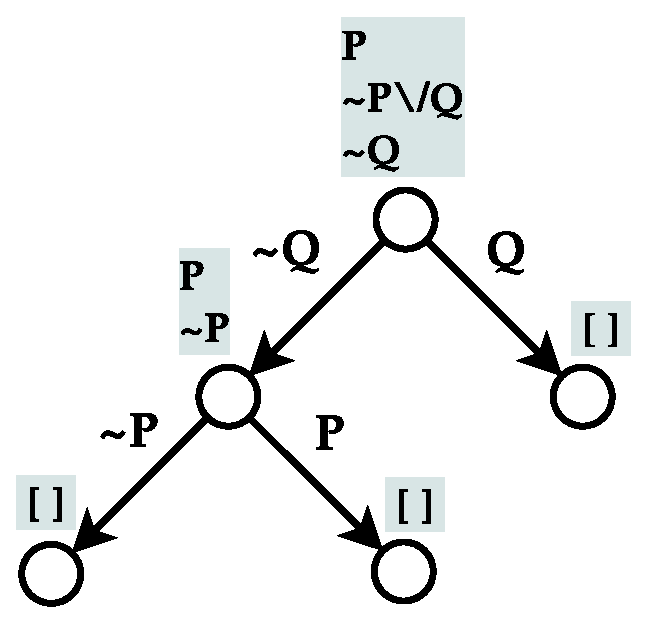
\includegraphics[width=0.85\textwidth]{sat.eps}

        $P \land (\lnot P \lor Q) \land \lnot Q$
      \end{column}

    \end{columns}

  \end{block}
\end{frame}

\begin{frame}[fragile]
  \begin{block}{EUF求解}
    求解变元或函数的相等关系
  \end{block}
  \begin{block}{}
    \begin{columns}
      
      \begin{column}{0.55\textwidth}
         \begin{itemize}
         \item 基于并查集(Union-Find Set)
         \item 使用等词的自反、对称、传递律及函数的等价替换律
         \end{itemize}
      \end{column}

      \begin{column}{0.40\textwidth}
        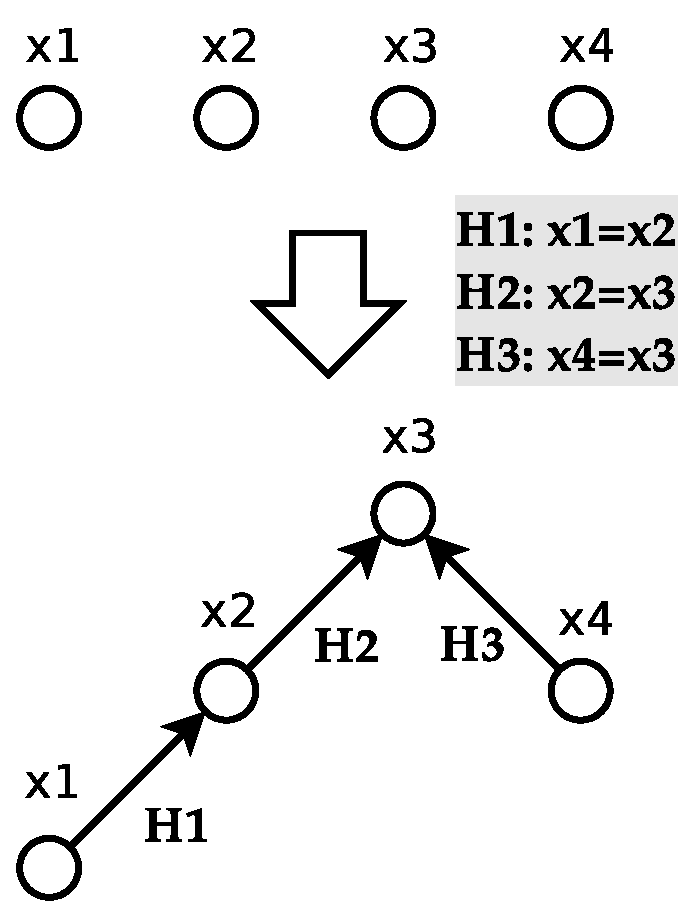
\includegraphics[width=0.85\textwidth]{euf.eps}
      \end{column}

    \end{columns}

  \end{block}
\end{frame}

\begin{frame}[fragile]
  \begin{block}{LIA求解}
      求解线性不等式组
  \end{block}
  \begin{block}{}
    \begin{columns}
      
      \begin{column}{0.45\textwidth}
        \begin{itemize}
         \item 基于线性规划理论
         \item 单纯形法(Simplex Method)
         \item 可用下述定理构造Coq证明
        \end{itemize}
      \end{column}

      \begin{column}{0.45\textwidth}
        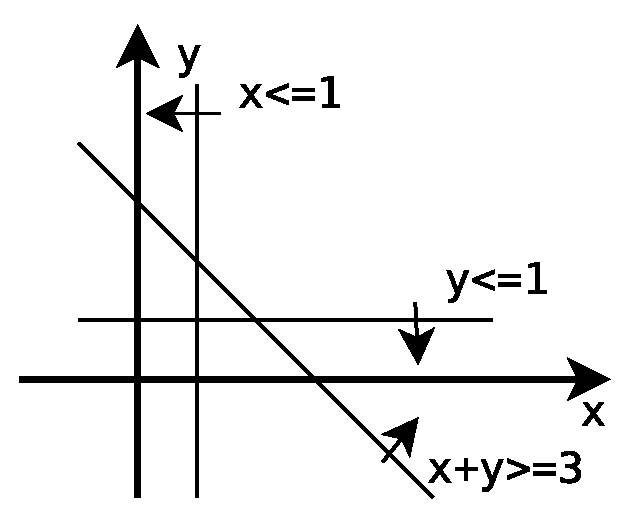
\includegraphics[width=0.85\textwidth]{arith.eps}
      \end{column}

    \end{columns}

  \end{block}

  \begin{block}{}
           $$x \leq a \land x > a \rightarrow \mathrm{False}$$
           $$
           (x < a \rightarrow \mathrm{False}) \land
           (x = a \rightarrow \mathrm{False}) \land
           (x > a \rightarrow \mathrm{False}) \rightarrow \mathrm{False}
           $$
  \end{block}
\end{frame}

\section{下一步的计划}
\begin{frame}[fragile]
  \begin{block}{完成LIA的证明生成}
    主要难点在于表达式化简的证明生成
  \end{block}

  \begin{block}{完成分离逻辑证明}
    根据时间量力而行
  \end{block}

  \begin{block}{完成毕业论文}
  \end{block}
\end{frame}
\end{document}
